\section{The RationalGRL Methodology and Tool}
\label{sect:methodology+tool}

In previous sections, we have shown how the RationalGRL framework can capture stakeholders discussions, and how interactions between two types of reasoning, practical reasoning and goal modeling, leads to two interlinked models, RationalGRL and GRL models. The previous section contained a formalization of RationalGRL, which forms the starting point of this section. In this section we clarify how practitioners can actually use the RationalGRL framework by proposing a methodology (\textbf{requirement 4}) and discussing a prototype RationalGRL tool (\textbf{requirement 5}).

\subsection{RationalGRL Methodology}
\label{sect:methodology} 

We propose the methodology shown in Figure~\ref{fig:rationalgrl-methodology} to develop a RationalGRL model, a version of which was presented at the 2017 iStar workshop \cite{ghanavatiMethodology}. Here we assume that the initial GRL models have been created based on the requirements specification documents and the discussions of the stakeholders. The rest of the steps are as follows:

\textbf{(1) Instantiate Argument Schemes (AS)} -- In this step, we start from the list of arguments schemes (Table~\ref{table:argument-schemes}). Whilst discussing the requirements, we select schemes from the list and instantiate them to form arguments for GRL IEs or links. In this way we build the GRL model by introducing new GRL elements (\textsf{INTRO}). For example, an argument scheme can be "Goal \emph{G} contributes to softgoal \emph{S}". When an argument scheme is instantiated, it corresponds to an argument for or against part of a goal model.

\textbf{(2) Answer Critical Questions (CQs)} -- After building or modifying the initial GRL model, we ask the relevant critical questions. Since each element in the GRL model corresponds to an instantiated scheme, we can look at Table~\ref{table:argument-schemes}) to see which questions are relevant given our GRL model. For example, for the argument scheme, "Goal \emph{G} contributes to softgoal \emph{S}", there are two critical questions as follows:  \emph{Does the goal contributes to the softgoal?} and \emph{Does the goal contributes to some other softgoals?}. When the analyst answers  a critical question, a new argument scheme may be instantiated. This is done in step (3) when the operation INTRO is executed.

\textbf{(3) Decide on Intentional Elements and their Relationships} -- By answering a critical question, one of the three operations (\textsf{INTRO}, \textsf{DISABLE} or \textsf{REPLACE}) is applied to the GRL model. Any of these operations impact the arguments and corresponding GRL intentional elements, modifying the initial GRL model into a RationalGRL model. Recall that \textsf{INTRO} means that 
a new argument scheme is created. That means, the current argument related to the critical question does not get attacked.  In the case of \textsf{DISABLE}, the intentional element or its related links are disabled in the model. \textsf{REPLACE} introduces a new argument and attacks the original argument at the same time. This means that the original element of the argument scheme is replaced with a new one.   

\textbf{(4) Modify GRL Models} -- Based on the RationalGRL model of step (3), the GRL model can be modified: 1) a new intentional element or a new link is introduced; 2) an existing intentional element or an existing link gets disabled (removed) from the model; or 3) an existing intentional element or link is replaced by a new one. This results in a new, modified GRL model, which can be used as the basis for another cycle of the methodology. 

We can continue these four steps until there is no more intentional element or link to analyze or we reach a satisfactory model. In the next section, we will give an example of how our tool can be used together with the methodology to build a GRL model.  

\begin{figure*}[t]
\centering
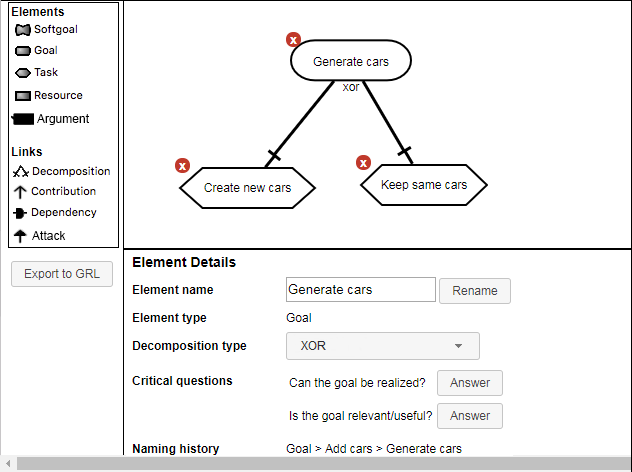
\includegraphics[scale=0.8]{img/tool/goal_details}
\caption{Overview of the RationalGRL tool}
\label{fig:tool:overview}
\end{figure*}


\subsection{The RationalGRL Tool}
\label{sect:tool}

The final requirement of our framework is that it has tool support (\textbf{requirement 5}). This is important for various reasons: i) although there are various approaches attempting to combine goal modeling with argumentation, we are not aware of existing tool support (see Section~\ref{sect:discussion}), ii) it allows us to do user tests in future research, exploring the difference between GRL and RationalGRL, iii) tool support is an excellent demonstration to show that our formal framework and algorithms actually work. In this section we briefly highlight some features of the tool, and we explain some of its current limitations. The tool can be accessed from:

\begin{quote}
\url{http://www.rationalgrl.com}
\end{quote}

\paragraph{Relation to jUCMNav} 

GRL is implemented in the open-source tool jUCMNav~\cite{jUCMNav}, which is actively maintained\footnote{\url{http://jucmnav.softwareengineering.ca/foswiki/ProjetSEG}}. jUCMNav currently has over 2,000 commits made by over 40 contributors, representing over 200,000 lines of code. jUCMNav is used actively in research, and the tool has been extended in many directions over the past few years, such as for modeling and analyzing security misuse cases~\cite{daramola2012ontology}, supporting activity theory \cite{georg2015synergy}, combined goal and feature model reasoning~\cite{liu2014combined}, and enterprise architecture modeling \cite{marosin-etal:caise2016}. Furthermore, jUCMNav includes Use Case modeling and contains various GRL evaluation algorithms with which the satisfiability of goals can be determined. 

The jUCMNav tool is implemented as an Eclipse plugin. While we aim to integrate our framework into jUCMNav in the future, a web-based version of RationalGRL (and GRL) is more suited for current purposes. Since RationalGRL does not make use of the many features of jUCMNav, we believe a light-weight version is sufficient for our current aims, and may benefit the community in general. Our tool is thus not meant to replace jUCMNav. For simplicity we have a web-based version, and it has the functionality to export to jUCMNav.

\paragraph{Tool overview} The RationalGRL tool is an open-source web-based Javascript application, which runs on all modern browsers. It is based on our formalization in Section~\ref{sect:formalframework} and provides export functionality to jUCMNav, using the translation algorithm (Algorithm~\ref{alg:translation:to-grl}). It contains all of the GRL elements and links, except for beliefs and actors. We have argued in Section~\ref{sect:background:grl} that arguments can be seen as an extension to beliefs, which is the reason why we did not implement them. Actors are also missing, but they will be added in the future.

When the tool starts, the user is presented with a screen as in Figure~\ref{fig:tool:overview}. This screen shows the palette of elements and links (top left pane), a canvas on which RationalGRL models can be built (top right pane), an `Export to GRL' button (bottom left pane), and a details pane of the currently selected elements (bottom right pane). Elements and links can be added to the canvas by selecting them on the left and clicking on the canvas, thus capturing the \textsf{INTRO} operation (Section~\ref{sect:formalframework:intro}). This makes it possible to build and modify GRL models using the tool. 

In total there are four different types of details panes, which we now explain in turn.

\paragraph{IE and links details pane} Figure~\ref{fig:tool:overview} shows the details pane for the goal `Generate cars'. The user can change the name of the IE by changing the name and clicking `Rename', which will update the naming history on the bottom of the pane. The naming history is (simplified) implementation of the \textsf{REPLACE} operation on IEs, since it is a very simple form of \emph{clarification}. The main difference with jUCMNav is that we have a renaming history, so the user can see which names the IE had prior to the current one. If the IE has decomposition links, the user can change the decomposition type as well. Each IE and link has a set of associated critical questions, which can be answered in the details pane by click on the button next to the question.

\paragraph{Critical question details pane} The details panel can be used to answer the critical questions of the RationalGRL framework (Table~\ref{table:argument-schemes}): Figure~\ref{fig:tool:overview}, for example, shows two critical questions for the goal IE ``Generate cars'', namely ``Can the goal be realized?'' (CQ3) and ``Is the goal relevant/useful?'' (CQ11). As an example, consider Figure~\ref{fig:tool:cqdetails}, where the softgoal ``Easy to use'' is questioned with the relevancy question (CQ11). It is possible to select the answer and provide an explanation for the answer. 

Assume that in the example of Figure~\ref{fig:tool:cqdetails} the user selects ``No'' and clicks the ``Answer question'' button. A new argument is then automatically created that attacks the softgoal and the details pane shows the critical question as answered (Figure~\ref{fig:tool:cqeffect}). This is an implementation of a \textsf{DISABLE} algorithm (Section~\ref{sect:formalframework:disable}) similar to Algorithm~\ref{alg:actor-not-relevant}: a new argument is added that attacks the existing argument. 

\paragraph{Argument details pane} It is also possible to attack arguments by adding an ``Argument'' element and an ``Attack'' link manually. Consider, for example, Figure~\ref{fig:tool:argument}. Here, a new argument ``Necessary'', which attacks the previously generated argument based on CQ11, has been added by the user. As the details pane shows, this new argument is not based on a CQ. It is further worth noting that it is possible to provide further a explanation in argument elements, allowing for more fine-grained rationalizations. 

\begin{figure}[t]
\centering
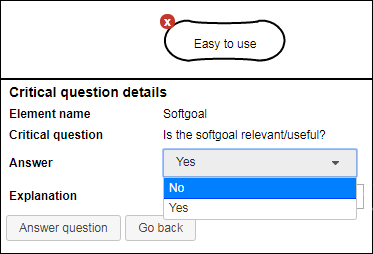
\includegraphics[width=0.8\columnwidth]{img/tool/details_softgoal}
\caption{Critical question details pane for ``Is the softgoal relevant/useful?''}
\label{fig:tool:cqdetails}
\end{figure}

\begin{figure}[b]
\centering
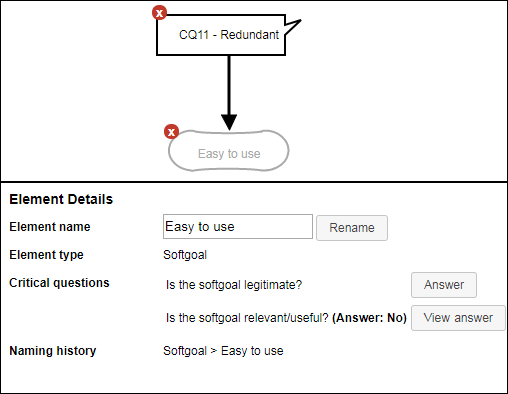
\includegraphics[width=\columnwidth]{img/tool/attack_softgoal}
\caption{Effect of answering CQ11: ``Is the softgoal relevant/useful?'' with ``No''}
\label{fig:tool:cqeffect}
\end{figure}

\paragraph{Argumentation semantics} The RationalGRL tool computes the acceptability of arguments on the fly. In the example of Figure~\ref{fig:tool:cqeffect}, the original (argument for) softgoal ``Easy to use'' is rejected because its only attacker ``CQ11 - Redundant'' is accepted. However, if we then attack ``CQ11 - Redundant'' with a new argument ``Necessary'', the original argument for ``Easy to use'' is again accepted because its only attacker is rejected  (Figure~\ref{fig:tool:argument}). Note that when computing the acceptability of arguments, the RationalGRL tool makes the assumption that there are no attack cycles in the model and that hence there is one unique preferred extension (cf. Section~\ref{sect:formalframework:rationalgrl}) -- if the user creates an attack cycle, an error message is shown. 

\begin{figure}[t]
\centering
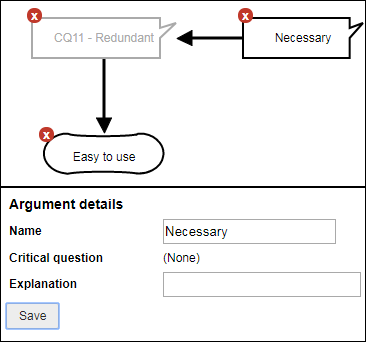
\includegraphics[width=0.8\columnwidth]{img/tool/reinstate_softgoal}
\caption{Attacking an argument with a generic argument ``Necessary''}
\label{fig:tool:argument}
\end{figure}

\paragraph{Argument schemes and critical questions} The tool contains more argument schemes and critical questions than those that we initial collected in Table~\ref{table:argument-schemes}. As we mentioned before, our table is not meant to be exhaustive, and it is straightforward to add more argument schemes and critical questions if necessary. For instance, the table does not contain critical questions for links between all IEs (e.g., a contribution link from a task to a goal does not occur in the table). In the tool, we have added critical questions to all links and IEs. We implemented an \emph{argument schemes database}, which is designed to be extended easily.


\paragraph{Export to jUCMNav} The tool implements the RationalGRL to GRL translation (Algorithm~\ref{alg:translation:to-grl}) through an export function. RationalGRL models built in the RationalGRL tool can be exported to the \texttt{.grl} file format, which can be imported in jUCMNav. Note that in order for the GRL models to be rendered correctly, we recommend using the Graphviz dot\footnote{\url{http://www.graphviz.org/}} as the auto-layout tool (this can be selected under ``Auto layout preferences'' when importing the file in jUCMNav).

Two examples of this export are provided in Appendix~\ref{sect:tool-screenshots}. Figure~\ref{fig:tool:figfrompaper} shows the model that was discussed earlier in this paper (Figure~\ref{fig:example-small3}) in the RationalGRL tool. Recall that translating this model to GRL provided us with the model in Figure~\ref{fig:example-small}. This is also what follows from our export: if we export the RationalGRL model and then import the resulting GRL model in jUCMNav, we get the model in Figure~\ref{fig:tool:figfrompaper1}, which is the same as Figure~\ref{fig:example-small}.

Our translation and export function uses the argument acceptability as a way of determining the GRL model. Take for example, the RationalGRL model in Figure~\ref{fig:tool:multipleattack}. A positive contribution is added from ``Keep same cars'' to ``Simple design''. More inportantly, an argument ``not enough CPU'' has been added to the model. This argument attacks the ``Realistic simulation'' softgoal and the ``Create new cars'' task, arguing that there is not enough processing power for either of these to be feasible in the traffic simulator. Now, if we export this to GRL, the GRL elements that are rejected or disabled (greyed out in Figure~\ref{fig:tool:multipleattack}) are not included. This can be seen in Figure~\ref{fig:tool:multipleattack1}, where the jUCMNav GRL model that was exported from the RationalGRL tool is shown. The pair of figures \ref{fig:tool:multipleattack} and \ref{fig:tool:multipleattack1} also nicely shows the added value of RationalGRL: Figure~\ref{fig:tool:multipleattack} shows that there can be a larger discussion and rationalization underlying even a fairly simple goal model such as the one in Figure~\ref{fig:tool:multipleattack1}. 

\paragraph{Limitations}
For usability purposes, the \textsf{REPLACE} operation has been implemented differently than in our formal framework (Section~\ref{sect:formalframework:disable}). In the formal framework, a \textsf{REPLACE} introduces a new argument that replaces (and therefore attacks) all previous arguments with the same identifier. Including \textsf{REPLACE} like this in the tool would mean that, when the name of an element is changed, we would need to render all the previous versions of the element on the canvas of the tool. Since this would quickly become very cumbersome, we decided to implement a naming history for each element. For example, in Figure~\ref{fig:tool:overview}, the goal ``Generate cars'' was previously named ``Add cars''. In this way, a history is kept of how an element name was clarified without cluttering the model canvas. This feature is currently very limited and can be extended in various was, for instance by changing the IE type. Similarly, the decomposition type can be changed in the details pane (Figure~\ref{fig:tool:overview}) without introducing new elements that attack the original ones (cf. Figure~\ref{fig:example-small3}, where the old decomposition type $AND$ of ``Generate traffic'' is shown as an explicit argument).